% Options for packages loaded elsewhere
\PassOptionsToPackage{unicode}{hyperref}
\PassOptionsToPackage{hyphens}{url}
%
\documentclass[
]{book}
\usepackage{amsmath,amssymb}
\usepackage{lmodern}
\usepackage{ifxetex,ifluatex}
\ifnum 0\ifxetex 1\fi\ifluatex 1\fi=0 % if pdftex
  \usepackage[T1]{fontenc}
  \usepackage[utf8]{inputenc}
  \usepackage{textcomp} % provide euro and other symbols
\else % if luatex or xetex
  \usepackage{unicode-math}
  \defaultfontfeatures{Scale=MatchLowercase}
  \defaultfontfeatures[\rmfamily]{Ligatures=TeX,Scale=1}
\fi
% Use upquote if available, for straight quotes in verbatim environments
\IfFileExists{upquote.sty}{\usepackage{upquote}}{}
\IfFileExists{microtype.sty}{% use microtype if available
  \usepackage[]{microtype}
  \UseMicrotypeSet[protrusion]{basicmath} % disable protrusion for tt fonts
}{}
\makeatletter
\@ifundefined{KOMAClassName}{% if non-KOMA class
  \IfFileExists{parskip.sty}{%
    \usepackage{parskip}
  }{% else
    \setlength{\parindent}{0pt}
    \setlength{\parskip}{6pt plus 2pt minus 1pt}}
}{% if KOMA class
  \KOMAoptions{parskip=half}}
\makeatother
\usepackage{xcolor}
\IfFileExists{xurl.sty}{\usepackage{xurl}}{} % add URL line breaks if available
\IfFileExists{bookmark.sty}{\usepackage{bookmark}}{\usepackage{hyperref}}
\hypersetup{
  pdftitle={Regression and ANOVA},
  pdfauthor={Justin Patterson},
  hidelinks,
  pdfcreator={LaTeX via pandoc}}
\urlstyle{same} % disable monospaced font for URLs
\usepackage{color}
\usepackage{fancyvrb}
\newcommand{\VerbBar}{|}
\newcommand{\VERB}{\Verb[commandchars=\\\{\}]}
\DefineVerbatimEnvironment{Highlighting}{Verbatim}{commandchars=\\\{\}}
% Add ',fontsize=\small' for more characters per line
\usepackage{framed}
\definecolor{shadecolor}{RGB}{248,248,248}
\newenvironment{Shaded}{\begin{snugshade}}{\end{snugshade}}
\newcommand{\AlertTok}[1]{\textcolor[rgb]{0.94,0.16,0.16}{#1}}
\newcommand{\AnnotationTok}[1]{\textcolor[rgb]{0.56,0.35,0.01}{\textbf{\textit{#1}}}}
\newcommand{\AttributeTok}[1]{\textcolor[rgb]{0.77,0.63,0.00}{#1}}
\newcommand{\BaseNTok}[1]{\textcolor[rgb]{0.00,0.00,0.81}{#1}}
\newcommand{\BuiltInTok}[1]{#1}
\newcommand{\CharTok}[1]{\textcolor[rgb]{0.31,0.60,0.02}{#1}}
\newcommand{\CommentTok}[1]{\textcolor[rgb]{0.56,0.35,0.01}{\textit{#1}}}
\newcommand{\CommentVarTok}[1]{\textcolor[rgb]{0.56,0.35,0.01}{\textbf{\textit{#1}}}}
\newcommand{\ConstantTok}[1]{\textcolor[rgb]{0.00,0.00,0.00}{#1}}
\newcommand{\ControlFlowTok}[1]{\textcolor[rgb]{0.13,0.29,0.53}{\textbf{#1}}}
\newcommand{\DataTypeTok}[1]{\textcolor[rgb]{0.13,0.29,0.53}{#1}}
\newcommand{\DecValTok}[1]{\textcolor[rgb]{0.00,0.00,0.81}{#1}}
\newcommand{\DocumentationTok}[1]{\textcolor[rgb]{0.56,0.35,0.01}{\textbf{\textit{#1}}}}
\newcommand{\ErrorTok}[1]{\textcolor[rgb]{0.64,0.00,0.00}{\textbf{#1}}}
\newcommand{\ExtensionTok}[1]{#1}
\newcommand{\FloatTok}[1]{\textcolor[rgb]{0.00,0.00,0.81}{#1}}
\newcommand{\FunctionTok}[1]{\textcolor[rgb]{0.00,0.00,0.00}{#1}}
\newcommand{\ImportTok}[1]{#1}
\newcommand{\InformationTok}[1]{\textcolor[rgb]{0.56,0.35,0.01}{\textbf{\textit{#1}}}}
\newcommand{\KeywordTok}[1]{\textcolor[rgb]{0.13,0.29,0.53}{\textbf{#1}}}
\newcommand{\NormalTok}[1]{#1}
\newcommand{\OperatorTok}[1]{\textcolor[rgb]{0.81,0.36,0.00}{\textbf{#1}}}
\newcommand{\OtherTok}[1]{\textcolor[rgb]{0.56,0.35,0.01}{#1}}
\newcommand{\PreprocessorTok}[1]{\textcolor[rgb]{0.56,0.35,0.01}{\textit{#1}}}
\newcommand{\RegionMarkerTok}[1]{#1}
\newcommand{\SpecialCharTok}[1]{\textcolor[rgb]{0.00,0.00,0.00}{#1}}
\newcommand{\SpecialStringTok}[1]{\textcolor[rgb]{0.31,0.60,0.02}{#1}}
\newcommand{\StringTok}[1]{\textcolor[rgb]{0.31,0.60,0.02}{#1}}
\newcommand{\VariableTok}[1]{\textcolor[rgb]{0.00,0.00,0.00}{#1}}
\newcommand{\VerbatimStringTok}[1]{\textcolor[rgb]{0.31,0.60,0.02}{#1}}
\newcommand{\WarningTok}[1]{\textcolor[rgb]{0.56,0.35,0.01}{\textbf{\textit{#1}}}}
\usepackage{longtable,booktabs,array}
\usepackage{calc} % for calculating minipage widths
% Correct order of tables after \paragraph or \subparagraph
\usepackage{etoolbox}
\makeatletter
\patchcmd\longtable{\par}{\if@noskipsec\mbox{}\fi\par}{}{}
\makeatother
% Allow footnotes in longtable head/foot
\IfFileExists{footnotehyper.sty}{\usepackage{footnotehyper}}{\usepackage{footnote}}
\makesavenoteenv{longtable}
\usepackage{graphicx}
\makeatletter
\def\maxwidth{\ifdim\Gin@nat@width>\linewidth\linewidth\else\Gin@nat@width\fi}
\def\maxheight{\ifdim\Gin@nat@height>\textheight\textheight\else\Gin@nat@height\fi}
\makeatother
% Scale images if necessary, so that they will not overflow the page
% margins by default, and it is still possible to overwrite the defaults
% using explicit options in \includegraphics[width, height, ...]{}
\setkeys{Gin}{width=\maxwidth,height=\maxheight,keepaspectratio}
% Set default figure placement to htbp
\makeatletter
\def\fps@figure{htbp}
\makeatother
\setlength{\emergencystretch}{3em} % prevent overfull lines
\providecommand{\tightlist}{%
  \setlength{\itemsep}{0pt}\setlength{\parskip}{0pt}}
\setcounter{secnumdepth}{5}
\usepackage{booktabs}
\usepackage{amsthm}
\usepackage{mathtools}
\usepackage{tabularx}
\usepackage{longtable}
\makeatletter
\def\thm@space@setup{%
  \thm@preskip=8pt plus 2pt minus 4pt
  \thm@postskip=\thm@preskip
}
\makeatother
\ifluatex
  \usepackage{selnolig}  % disable illegal ligatures
\fi
\usepackage[]{biblatex}
\addbibresource{book.bib}
\addbibresource{packages.bib}

\title{Regression and ANOVA}
\author{Justin Patterson}
\date{2021-06-09}

\begin{document}
\maketitle

{
\setcounter{tocdepth}{1}
\tableofcontents
}
\hypertarget{prerequisites}{%
\chapter*{Prerequisites}\label{prerequisites}}
\addcontentsline{toc}{chapter}{Prerequisites}

This project is meant to be a personal guide to ANOVA and regression. The scope of this project does not include time series analysis. Also, the focus will not be on designing experiments, but rather on analyzing the data from experiments which have already been conducted. To accomplish this, we will use simulated experimental data.

\textbf{Disclaimer}
This project was not written by an expert. That being said, I would appreciate any comments.

This book is written in \textbf{Markdown}. You can use anything that Pandoc's Markdown supports, e.g., a math equation \(a^2 + b^2 = c^2\).

The \textbf{bookdown} package can be installed from CRAN or Github:

\begin{Shaded}
\begin{Highlighting}[]
\FunctionTok{install.packages}\NormalTok{(}\StringTok{"bookdown"}\NormalTok{)}
\CommentTok{\# or the development version}
\CommentTok{\# devtools::install\_github("rstudio/bookdown")}
\end{Highlighting}
\end{Shaded}

Remember each Rmd file contains one and only one chapter, and a chapter is defined by the first-level heading \texttt{\#}.

To compile this example to PDF, you need XeLaTeX. You are recommended to install TinyTeX (which includes XeLaTeX): \url{https://yihui.name/tinytex/}.

\hypertarget{intro}{%
\chapter{Introduction}\label{intro}}

You can label chapter and section titles using \texttt{\{\#label\}} after them, e.g., we can reference Chapter \ref{intro}. If you do not manually label them, there will be automatic labels anyway, e.g., Chapter \ref{methods}.

Figures and tables with captions will be placed in \texttt{figure} and \texttt{table} environments, respectively.

\begin{Shaded}
\begin{Highlighting}[]
\FunctionTok{par}\NormalTok{(}\AttributeTok{mar =} \FunctionTok{c}\NormalTok{(}\DecValTok{4}\NormalTok{, }\DecValTok{4}\NormalTok{, .}\DecValTok{1}\NormalTok{, .}\DecValTok{1}\NormalTok{))}
\FunctionTok{plot}\NormalTok{(pressure, }\AttributeTok{type =} \StringTok{\textquotesingle{}b\textquotesingle{}}\NormalTok{, }\AttributeTok{pch =} \DecValTok{19}\NormalTok{)}
\end{Highlighting}
\end{Shaded}

\begin{figure}

{\centering 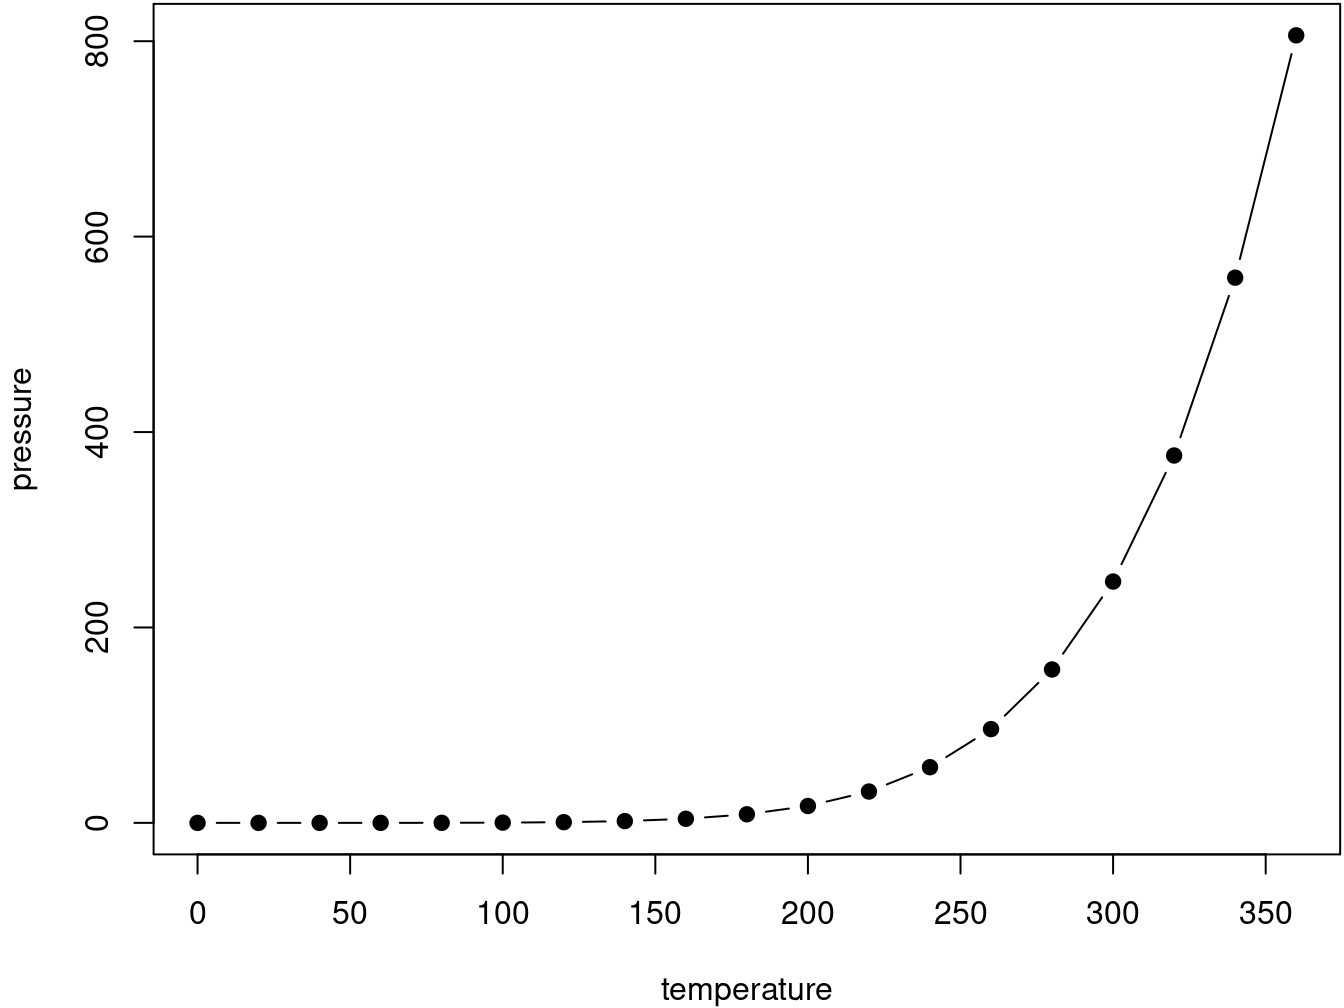
\includegraphics[width=0.8\linewidth]{ANOVA-and-Regression_files/figure-latex/nice-fig-1} 

}

\caption{Here is a nice figure!}\label{fig:nice-fig}
\end{figure}

Reference a figure by its code chunk label with the \texttt{fig:} prefix, e.g., see Figure \ref{fig:nice-fig}. Similarly, you can reference tables generated from \texttt{knitr::kable()}, e.g., see Table \ref{tab:nice-tab}.

\begin{Shaded}
\begin{Highlighting}[]
\NormalTok{knitr}\SpecialCharTok{::}\FunctionTok{kable}\NormalTok{(}
  \FunctionTok{head}\NormalTok{(iris, }\DecValTok{20}\NormalTok{), }\AttributeTok{caption =} \StringTok{\textquotesingle{}Here is a nice table!\textquotesingle{}}\NormalTok{,}
  \AttributeTok{booktabs =} \ConstantTok{TRUE}
\NormalTok{)}
\end{Highlighting}
\end{Shaded}

\begin{table}

\caption{\label{tab:nice-tab}Here is a nice table!}
\centering
\begin{tabular}[t]{rrrrl}
\toprule
Sepal.Length & Sepal.Width & Petal.Length & Petal.Width & Species\\
\midrule
5.1 & 3.5 & 1.4 & 0.2 & setosa\\
4.9 & 3.0 & 1.4 & 0.2 & setosa\\
4.7 & 3.2 & 1.3 & 0.2 & setosa\\
4.6 & 3.1 & 1.5 & 0.2 & setosa\\
5.0 & 3.6 & 1.4 & 0.2 & setosa\\
\addlinespace
5.4 & 3.9 & 1.7 & 0.4 & setosa\\
4.6 & 3.4 & 1.4 & 0.3 & setosa\\
5.0 & 3.4 & 1.5 & 0.2 & setosa\\
4.4 & 2.9 & 1.4 & 0.2 & setosa\\
4.9 & 3.1 & 1.5 & 0.1 & setosa\\
\addlinespace
5.4 & 3.7 & 1.5 & 0.2 & setosa\\
4.8 & 3.4 & 1.6 & 0.2 & setosa\\
4.8 & 3.0 & 1.4 & 0.1 & setosa\\
4.3 & 3.0 & 1.1 & 0.1 & setosa\\
5.8 & 4.0 & 1.2 & 0.2 & setosa\\
\addlinespace
5.7 & 4.4 & 1.5 & 0.4 & setosa\\
5.4 & 3.9 & 1.3 & 0.4 & setosa\\
5.1 & 3.5 & 1.4 & 0.3 & setosa\\
5.7 & 3.8 & 1.7 & 0.3 & setosa\\
5.1 & 3.8 & 1.5 & 0.3 & setosa\\
\bottomrule
\end{tabular}
\end{table}

You can write citations, too. For example, we are using the \textbf{bookdown} package \autocite{R-bookdown} in this sample book, which was built on top of R Markdown and \textbf{knitr} \autocite{xie2015}.

\hypertarget{literature}{%
\chapter{Literature}\label{literature}}

Here is a review of existing methods.

\hypertarget{methods}{%
\chapter{Methods}\label{methods}}

We describe our methods in this chapter.

\hypertarget{applications}{%
\chapter{Applications}\label{applications}}

Some \emph{significant} applications are demonstrated in this chapter.

\hypertarget{example-one}{%
\section{Example one}\label{example-one}}

\hypertarget{example-two}{%
\section{Example two}\label{example-two}}

\hypertarget{final-words}{%
\chapter{Final Words}\label{final-words}}

We have finished a nice book.

\hypertarget{anova-tutorial}{%
\chapter{ANOVA Tutorial}\label{anova-tutorial}}

\begin{Shaded}
\begin{Highlighting}[]
\FunctionTok{library}\NormalTok{(cellWise)}
\FunctionTok{library}\NormalTok{(knitr)}
\NormalTok{opts\_chunk}\SpecialCharTok{$}\FunctionTok{set}\NormalTok{(}\AttributeTok{tidy.opts=}\FunctionTok{list}\NormalTok{(}\AttributeTok{width.cutoff=}\DecValTok{50}\NormalTok{),}\AttributeTok{tidy=}\ConstantTok{TRUE}\NormalTok{)}
\end{Highlighting}
\end{Shaded}

\hypertarget{step-1-make-up-data}{%
\section{Step 1: Make up Data}\label{step-1-make-up-data}}

\begin{Shaded}
\begin{Highlighting}[]
\CommentTok{\# dataset1}
\end{Highlighting}
\end{Shaded}

\hypertarget{checking-the-assumptions}{%
\section{Checking the Assumptions}\label{checking-the-assumptions}}

After running your ANOVA, check that the assumptions about the errors
are met so that you can do statistical inference. Those assumptions are:

\begin{enumerate}
\def\labelenumi{\arabic{enumi}.}
\tightlist
\item
  \(\text{E}(\epsilon_{ij})=0,\ \text{Var}(\epsilon_{ij})=\sigma_{i}^2 < \infty,\ \text{for all }i, j.\)
\item
  The \(\epsilon_{ij}\) are mutually independent and normally
  distributed.
\item
  \(\sigma_{i}^2=\sigma^2\ \text{for all } i.\)
\end{enumerate}

\hypertarget{checking-assumption-1}{%
\subsection{Checking Assumption 1}\label{checking-assumption-1}}

\hypertarget{assumption-1-was-violated.}{%
\subsection{Assumption 1 was violated.}\label{assumption-1-was-violated.}}

\hypertarget{checking-assumption-2}{%
\subsection{Checking Assumption 2}\label{checking-assumption-2}}

\hypertarget{assumption-2-was-violated.}{%
\subsection{Assumption 2 was violated.}\label{assumption-2-was-violated.}}

\hypertarget{checking-assumption-3}{%
\subsection{Checking Assumption 3}\label{checking-assumption-3}}

\hypertarget{assumption-3-was-violated.}{%
\subsection{Assumption 3 was violated.}\label{assumption-3-was-violated.}}

A variance-stabilizing transformation of the response variable may help.

\begin{Shaded}
\begin{Highlighting}[]
\FunctionTok{data}\NormalTok{(}\StringTok{"data\_mortality"}\NormalTok{)}
\NormalTok{transformed\_response }\OtherTok{=} \FunctionTok{transfo}\NormalTok{(data\_mortality, }\AttributeTok{prestandardize =} \ConstantTok{FALSE}\NormalTok{)}
\end{Highlighting}
\end{Shaded}

\begin{verbatim}
##  
##  The input data has 198 rows and 91 columns.
\end{verbatim}

\begin{Shaded}
\begin{Highlighting}[]
\FunctionTok{hist}\NormalTok{(data\_mortality[, }\DecValTok{1}\NormalTok{])}
\end{Highlighting}
\end{Shaded}

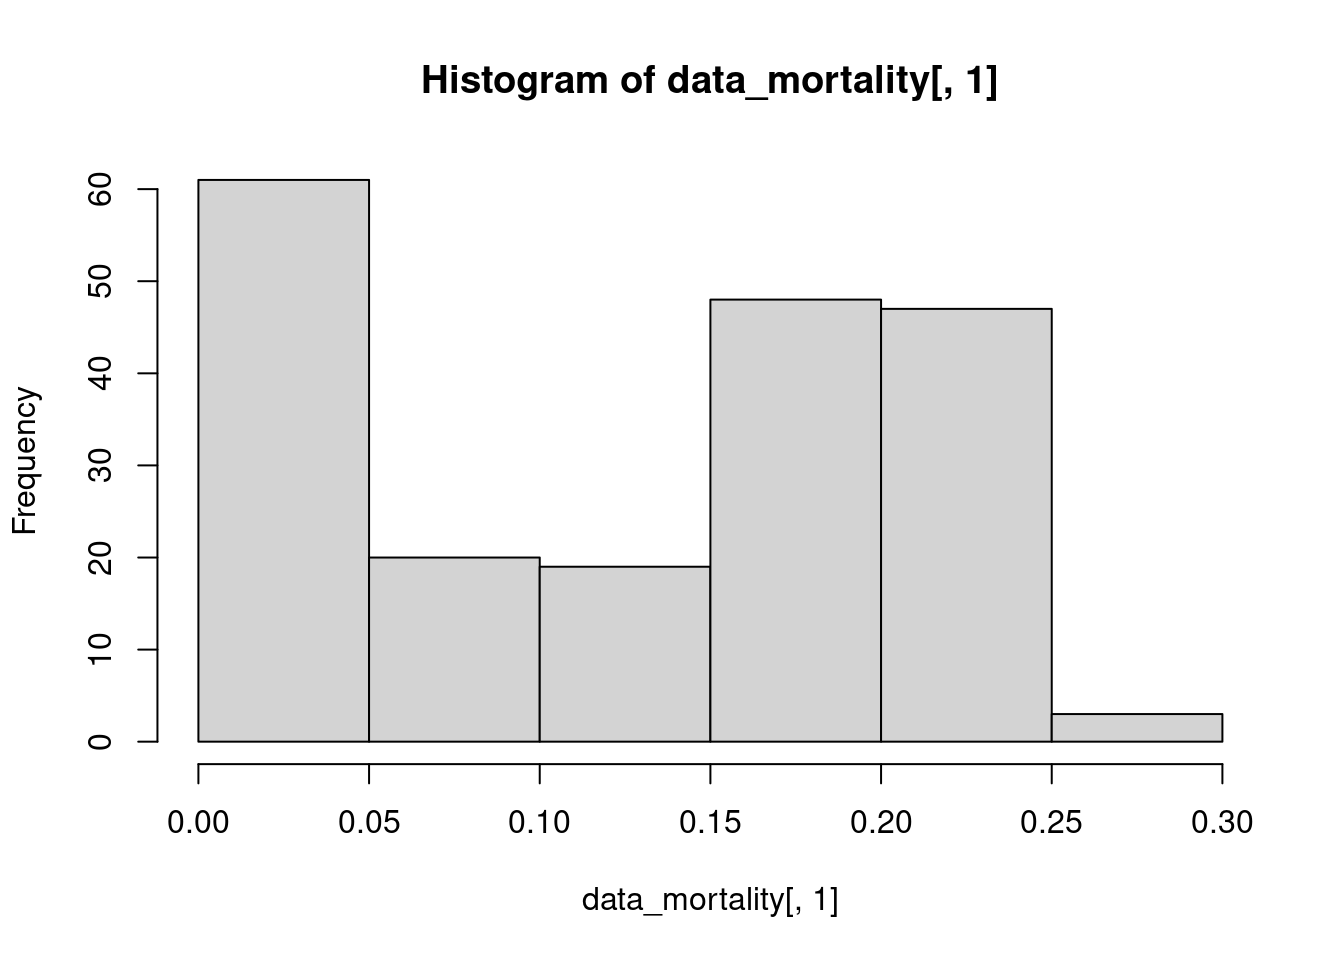
\includegraphics{ANOVA-and-Regression_files/figure-latex/unnamed-chunk-5-1.pdf}

\begin{Shaded}
\begin{Highlighting}[]
\FunctionTok{hist}\NormalTok{(transformed\_response}\SpecialCharTok{$}\NormalTok{Xt[, }\DecValTok{1}\NormalTok{])}
\end{Highlighting}
\end{Shaded}

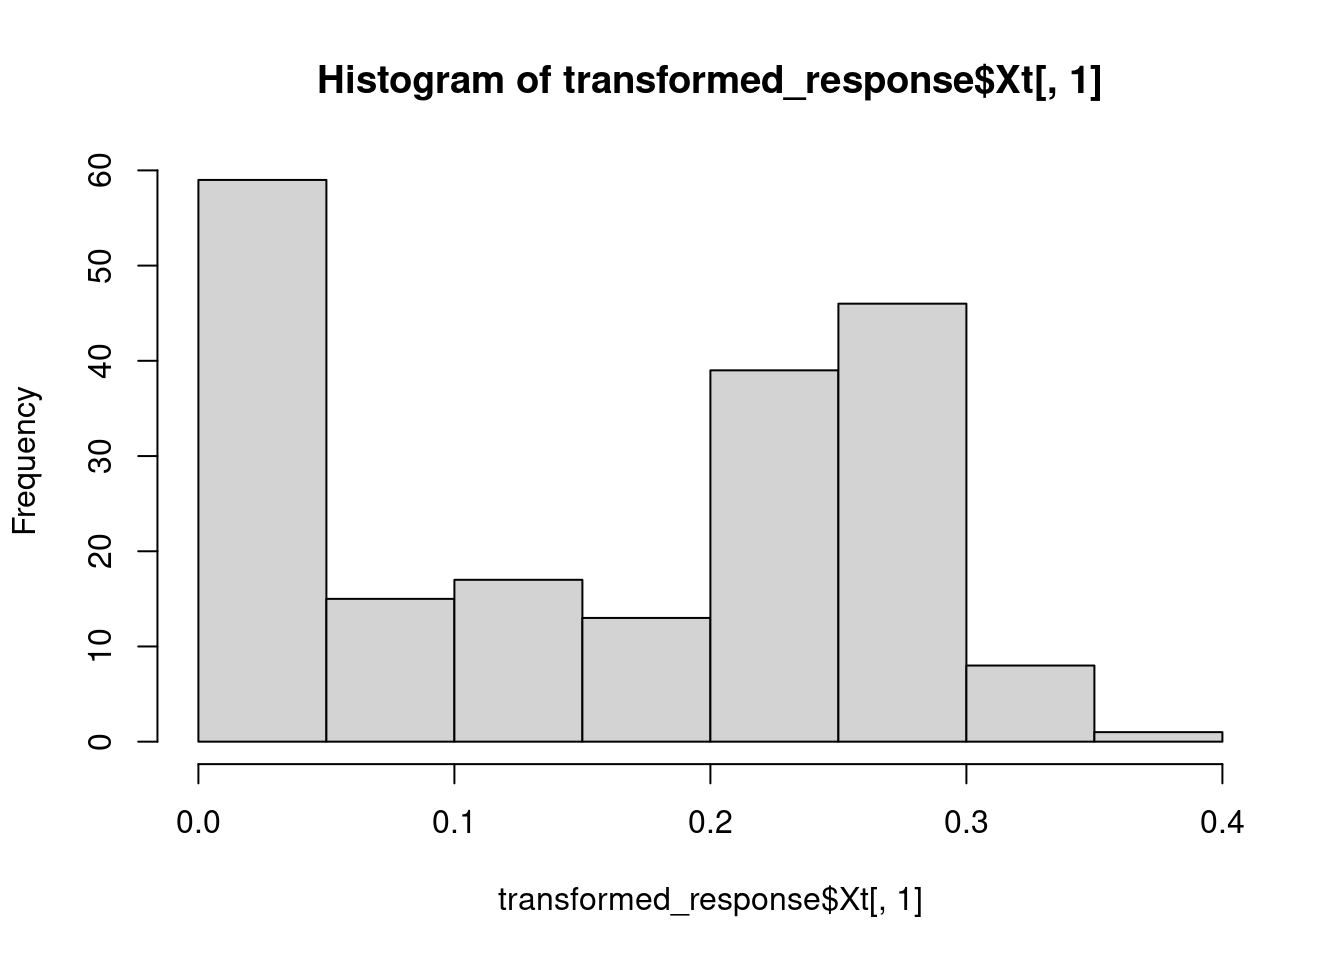
\includegraphics{ANOVA-and-Regression_files/figure-latex/unnamed-chunk-5-2.pdf}

\begin{Shaded}
\begin{Highlighting}[]
\FunctionTok{shapiro.test}\NormalTok{(data\_mortality[, }\DecValTok{1}\NormalTok{])}
\end{Highlighting}
\end{Shaded}

\begin{verbatim}
## 
##  Shapiro-Wilk normality test
## 
## data:  data_mortality[, 1]
## W = 0.86877, p-value = 4.552e-12
\end{verbatim}

\begin{Shaded}
\begin{Highlighting}[]
\FunctionTok{shapiro.test}\NormalTok{(transformed\_response}\SpecialCharTok{$}\NormalTok{Xt[, }\DecValTok{1}\NormalTok{])}
\end{Highlighting}
\end{Shaded}

\begin{verbatim}
## 
##  Shapiro-Wilk normality test
## 
## data:  transformed_response$Xt[, 1]
## W = 0.88041, p-value = 1.968e-11
\end{verbatim}

\hypertarget{regression-and-categorical-variables}{%
\section{Regression and Categorical Variables}\label{regression-and-categorical-variables}}

\begin{Shaded}
\begin{Highlighting}[]
\FunctionTok{library}\NormalTok{(tidymodels)}
\end{Highlighting}
\end{Shaded}

\begin{verbatim}
## Registered S3 method overwritten by 'tune':
##   method                   from   
##   required_pkgs.model_spec parsnip
\end{verbatim}

\begin{verbatim}
## -- Attaching packages -------------------------------------- tidymodels 0.1.3 --
\end{verbatim}

\begin{verbatim}
## v broom        0.7.6      v recipes      0.1.16
## v dials        0.0.9      v rsample      0.1.0 
## v dplyr        1.0.6      v tibble       3.1.2 
## v ggplot2      3.3.3      v tidyr        1.1.3 
## v infer        0.5.4      v tune         0.1.5 
## v modeldata    0.1.0      v workflows    0.2.2 
## v parsnip      0.1.6      v workflowsets 0.0.2 
## v purrr        0.3.4      v yardstick    0.0.8
\end{verbatim}

\begin{verbatim}
## -- Conflicts ----------------------------------------- tidymodels_conflicts() --
## x purrr::discard() masks scales::discard()
## x dplyr::filter()  masks stats::filter()
## x dplyr::lag()     masks stats::lag()
## x recipes::step()  masks stats::step()
## * Use tidymodels_prefer() to resolve common conflicts.
\end{verbatim}

\begin{Shaded}
\begin{Highlighting}[]
\FunctionTok{library}\NormalTok{(ggplot2)}
\end{Highlighting}
\end{Shaded}

There is a profound connection between linear regression and ANOVA. In
order to see this, you have to understand that the categorical variables
of an ANOVA can be coded with numbers, which allows them to be used in a
linear regression model. Let us recall \autocite{LinearMod} the multiple linear
regression model.

Given a random sample of \(n\) observations
\((Y_{i}, X_{i1}, . . ., X_{ip}),\ i=1,...,n\), the basic multiple linear regression model is

\[
Y_{i}=\beta_0+\beta_1X_{i1}+...+\beta_pX_{ip}+\epsilon_i,\quad i=1,...,n
\]

where each \(\epsilon_i\) is a random variable with a mean of \(0\). In
matrix form, this can be written as

\[
\begin{bmatrix}
Y_1\\
Y_2\\
\vdots\\
Y_n
\end{bmatrix}
= 
\begin{bmatrix}
1 & X_{1,1} & X_{1,2} & \dots & X_{1, p}\\
1 & X_{2,1} & X_{2,2} & \dots & X_{2, p}\\
\vdots & \vdots & \vdots & \ddots & \vdots\\
1 & X_{n,1} & X_{n,2} & \dots & X_{n, p}\\
\end{bmatrix}
\begin{bmatrix}
\beta_0\\
\beta_1\\
\vdots\\
\beta_p\\
\end{bmatrix}
+
\begin{bmatrix}
\epsilon_0\\
\epsilon_1\\
\vdots\\
\epsilon_n\\
\end{bmatrix}
\]

Here, the \(X_{i,j}\) represent our coded categorical variables. These
categorical variables are coded according to the hypotheses of interest.
In many cases, the coding is done so that the newly coded variables are
contrasts of the old categorical variables.

A contrast is a linear combination of variables such that the
coefficients sum to 0.
\[\sum_i{a_i\theta_i}\quad\text{such that}\quad\sum_i{a_i}=0\]

Unlike in ANOVA, in regression, it is best to use coding schemes based
on orthogonal and fractional contrasts. Orthogonal contrasts are a set
of contrasts in which, for any distinct pair, the sum of the
cross-products of the coefficients is 0.
\[
\sum_i{a_ib_i}=0
\]

I believe that a fractional contrast is such that
\[
\sum_i{|a_i|}=2
\]

Categorical variable coding schemes can be easily expressed in a matrix
format. The convention is to have the old categorical variables as the
row headers and the newly coded variables as the column headers. In such
a matrix, the \([c_{ij}]\) entry indicates the value of the \(j^{th}\) level
of the new variable for the \(i^{th}\) level of the old variable. Here is
an example of such a matrix constructed using orthogonal and fractional
contrasts.

\begin{Shaded}
\begin{Highlighting}[]
\NormalTok{(}\AttributeTok{contr\_mat =} \FunctionTok{matrix}\NormalTok{(}\AttributeTok{data =} \FunctionTok{c}\NormalTok{(}\DecValTok{1}\NormalTok{, }\DecValTok{0}\NormalTok{, }\SpecialCharTok{{-}}\DecValTok{1}\NormalTok{, }\FloatTok{0.5}\NormalTok{, }\SpecialCharTok{{-}}\DecValTok{1}\NormalTok{, }\FloatTok{0.5}\NormalTok{),}
    \AttributeTok{nrow =} \DecValTok{3}\NormalTok{, }\AttributeTok{ncol =} \DecValTok{2}\NormalTok{))}
\end{Highlighting}
\end{Shaded}

\begin{verbatim}
##      [,1] [,2]
## [1,]    1  0.5
## [2,]    0 -1.0
## [3,]   -1  0.5
\end{verbatim}

Interpreting this coding scheme in the context of our linear model, we
see that

\[
\begin{aligned}
E(Y_i|X_{i1}=1,X_{i2}=\tfrac{1}{2}) &= \beta_0+\beta_1+\tfrac{1}{2}\beta_2 &= \mu_1 \\
E(Y_i|X_{i1}=0,X_{i2}=-1) &= \beta_0-\beta_2 &= \mu_2\\
E(Y_i|X_{i1}=-1,X_{i2}=\tfrac{1}{2}) &= \beta_0-\beta_1+\tfrac{1}{2}\beta_2 &= \mu_3
\end{aligned}
\]

or, in matrix format,
\[
\begin{bmatrix}
1 & 1 & \tfrac{1}{2} \\
1 & 0 & -1 \\
1 & -1 & \tfrac{1}{2}
\end{bmatrix}
\begin{bmatrix}
\beta_0 \\
\beta_1  \\
\beta_2 
\end{bmatrix}
=
\begin{bmatrix}
\mu_1 \\
\mu_2  \\
\mu_3 
\end{bmatrix}
\]

We can solve this for \(\boldsymbol{\beta}\) for interpretation's sake.

\begin{Shaded}
\begin{Highlighting}[]
\FunctionTok{solve}\NormalTok{(}\FunctionTok{cbind}\NormalTok{(}\FunctionTok{rep}\NormalTok{(}\DecValTok{1}\NormalTok{, }\FunctionTok{nrow}\NormalTok{(contr\_mat)), contr\_mat))}
\end{Highlighting}
\end{Shaded}

\begin{verbatim}
##           [,1]       [,2]       [,3]
## [1,] 0.3333333  0.3333333  0.3333333
## [2,] 0.5000000  0.0000000 -0.5000000
## [3,] 0.3333333 -0.6666667  0.3333333
\end{verbatim}

\begin{tabularx}{\textwidth}{r c c X}
\(\beta_0 =\) &\(\tfrac{\mu_1+\mu_2+\mu_3}{3}\) &\(=\) &grand mean response \\
\(2\beta_1 =\) &\(\mu_1 - \mu_3\) &\(=\) &difference in the mean response between levels 1 and 3 of the old categorical variable \\
\(\tfrac{3}{2}\beta_2 =\) &\(\tfrac{\mu_1+\mu_3}{2} - \mu_2\) &\(=\) &difference in the mean response between level 2 and the average of levels 1 and 3 of the old categorical variable
\end{tabularx}

Let's look at another contrast matrix and see if we can interpret it.

\begin{Shaded}
\begin{Highlighting}[]
\FunctionTok{contr.helmert}\NormalTok{(}\AttributeTok{n =} \DecValTok{3}\NormalTok{)}
\end{Highlighting}
\end{Shaded}

\begin{verbatim}
##   [,1] [,2]
## 1   -1   -1
## 2    1   -1
## 3    0    2
\end{verbatim}

\begin{Shaded}
\begin{Highlighting}[]
\FunctionTok{solve}\NormalTok{(}\FunctionTok{cbind}\NormalTok{(}\FunctionTok{rep}\NormalTok{(}\DecValTok{1}\NormalTok{, }\DecValTok{3}\NormalTok{), }\FunctionTok{contr.helmert}\NormalTok{(}\AttributeTok{n =} \DecValTok{3}\NormalTok{)))}
\end{Highlighting}
\end{Shaded}

\begin{verbatim}
##               1          2         3
## [1,]  0.3333333  0.3333333 0.3333333
## [2,] -0.5000000  0.5000000 0.0000000
## [3,] -0.1666667 -0.1666667 0.3333333
\end{verbatim}

\begin{tabularx}{\textwidth}{r c c X}
\(\beta_0 =\) &\(\tfrac{\mu_1+\mu_2+\mu_3}{3}\) &\(=\) &grand mean response \\
\(2\beta_1 =\) &\(\mu_2 - \mu_1\) &\(=\) &difference in the mean response between levels 2 \& 1 of the old categorical variable \\
\(3\beta_2 =\) &\(\mu_3 - \tfrac{\mu_1+\mu_2}{2}\) &\(=\) &difference in the mean response between level 3 and the average of levels 1 and 2 of the old categorical variable
\end{tabularx}

Perhaps you have heard of polynomial regression? Polynomial regression
is just a special case of linear regression in a different basis. In
polynomial regression, (just like multiple linear regression) if you use
all of your explanatory variables, then you will likely get
multi-collinearity problems.

\begin{Shaded}
\begin{Highlighting}[]
\FunctionTok{contr.poly}\NormalTok{(}\AttributeTok{n =} \DecValTok{3}\NormalTok{)}
\end{Highlighting}
\end{Shaded}

\begin{verbatim}
##                 .L         .Q
## [1,] -7.071068e-01  0.4082483
## [2,] -7.850462e-17 -0.8164966
## [3,]  7.071068e-01  0.4082483
\end{verbatim}

\begin{Shaded}
\begin{Highlighting}[]
\NormalTok{(}\AttributeTok{A =} \FunctionTok{solve}\NormalTok{(}\FunctionTok{cbind}\NormalTok{(}\FunctionTok{rep}\NormalTok{(}\DecValTok{1}\NormalTok{, }\DecValTok{3}\NormalTok{), }\FunctionTok{contr.poly}\NormalTok{(}\AttributeTok{n =} \DecValTok{3}\NormalTok{))))}
\end{Highlighting}
\end{Shaded}

\begin{verbatim}
##          [,1]       [,2]      [,3]
##     0.3333333  0.3333333 0.3333333
## .L -0.7071068  0.0000000 0.7071068
## .Q  0.4082483 -0.8164966 0.4082483
\end{verbatim}

The first matrix shows how to code the levels of your categorical
variable and the second matrix is used for interpretation.

\begin{tabularx}{\textwidth}{r c c X}
\(\beta_0 =\) &\(\tfrac{\mu_1+\mu_2+\mu_3}{3}\) &\(=\) &grand mean response \\
\(\beta_1 =\) &\(-0.707\mu_1 + 0.707\mu_3\) &\(=\) &measure of a linear trend in the mean response \\
\(\beta_2 =\) &\(0.408 \mu_3 - 0.816 \mu_2 + 0.408 \mu_3\) &\(=\) &measure of a quadratic trend in the mean response
\end{tabularx}

For example, we can test whether the difference between the means from
two populations are equal by doing a linear regression or an ANOVA.

Let's make up some data and try it!

\begin{Shaded}
\begin{Highlighting}[]
\FunctionTok{source}\NormalTok{(}\FunctionTok{file.path}\NormalTok{(}\StringTok{"src"}\NormalTok{, }\StringTok{"fabricate.R"}\NormalTok{))}
\NormalTok{design }\OtherTok{=} \FunctionTok{data.frame}\NormalTok{(}\AttributeTok{group =} \FunctionTok{c}\NormalTok{(}\DecValTok{0}\NormalTok{, }\DecValTok{1}\NormalTok{), }\AttributeTok{n =} \FunctionTok{c}\NormalTok{(}\DecValTok{10}\NormalTok{, }\DecValTok{10}\NormalTok{))}
\NormalTok{data1 }\OtherTok{=} \FunctionTok{fabricate}\NormalTok{(}\AttributeTok{flr =}\NormalTok{ design)}
\end{Highlighting}
\end{Shaded}

Let's check out our data.

\begin{Shaded}
\begin{Highlighting}[]
\CommentTok{\# Make a linear model}
\NormalTok{data1\_lm\_independent\_samples }\OtherTok{=} \FunctionTok{lm}\NormalTok{(response }\SpecialCharTok{\textasciitilde{}}\NormalTok{ group,}
    \AttributeTok{data =}\NormalTok{ data1)}
\CommentTok{\# plot}
\FunctionTok{ggplot}\NormalTok{(}\AttributeTok{data =}\NormalTok{ data1, }\FunctionTok{aes}\NormalTok{(}\AttributeTok{x =}\NormalTok{ group, }\AttributeTok{y =}\NormalTok{ response, }\AttributeTok{color =} \FunctionTok{factor}\NormalTok{(group))) }\SpecialCharTok{+}
    \FunctionTok{geom\_boxplot}\NormalTok{() }\SpecialCharTok{+} \FunctionTok{geom\_jitter}\NormalTok{(}\AttributeTok{height =} \DecValTok{0}\NormalTok{, }\AttributeTok{width =} \FloatTok{0.1}\NormalTok{) }\SpecialCharTok{+}
    \FunctionTok{geom\_abline}\NormalTok{(}\AttributeTok{intercept =}\NormalTok{ data1\_lm\_independent\_samples}\SpecialCharTok{$}\NormalTok{coefficients[}\DecValTok{1}\NormalTok{],}
        \AttributeTok{slope =}\NormalTok{ data1\_lm\_independent\_samples}\SpecialCharTok{$}\NormalTok{coefficients[}\DecValTok{2}\NormalTok{]) }\SpecialCharTok{+}
    \FunctionTok{labs}\NormalTok{(}\AttributeTok{title =} \StringTok{"Group Comparison from a Regression Standpoint"}\NormalTok{,}
        \AttributeTok{color =} \StringTok{"Group"}\NormalTok{, }\AttributeTok{x =} \StringTok{"Group"}\NormalTok{, }\AttributeTok{y =} \StringTok{"Response"}\NormalTok{) }\SpecialCharTok{+}
    \FunctionTok{scale\_x\_discrete}\NormalTok{(}\AttributeTok{limits =} \FunctionTok{c}\NormalTok{(}\DecValTok{0}\NormalTok{, }\DecValTok{1}\NormalTok{))}
\end{Highlighting}
\end{Shaded}

\begin{verbatim}
## Warning: Continuous limits supplied to discrete scale.
## Did you mean `limits = factor(...)` or `scale_*_continuous()`?
\end{verbatim}

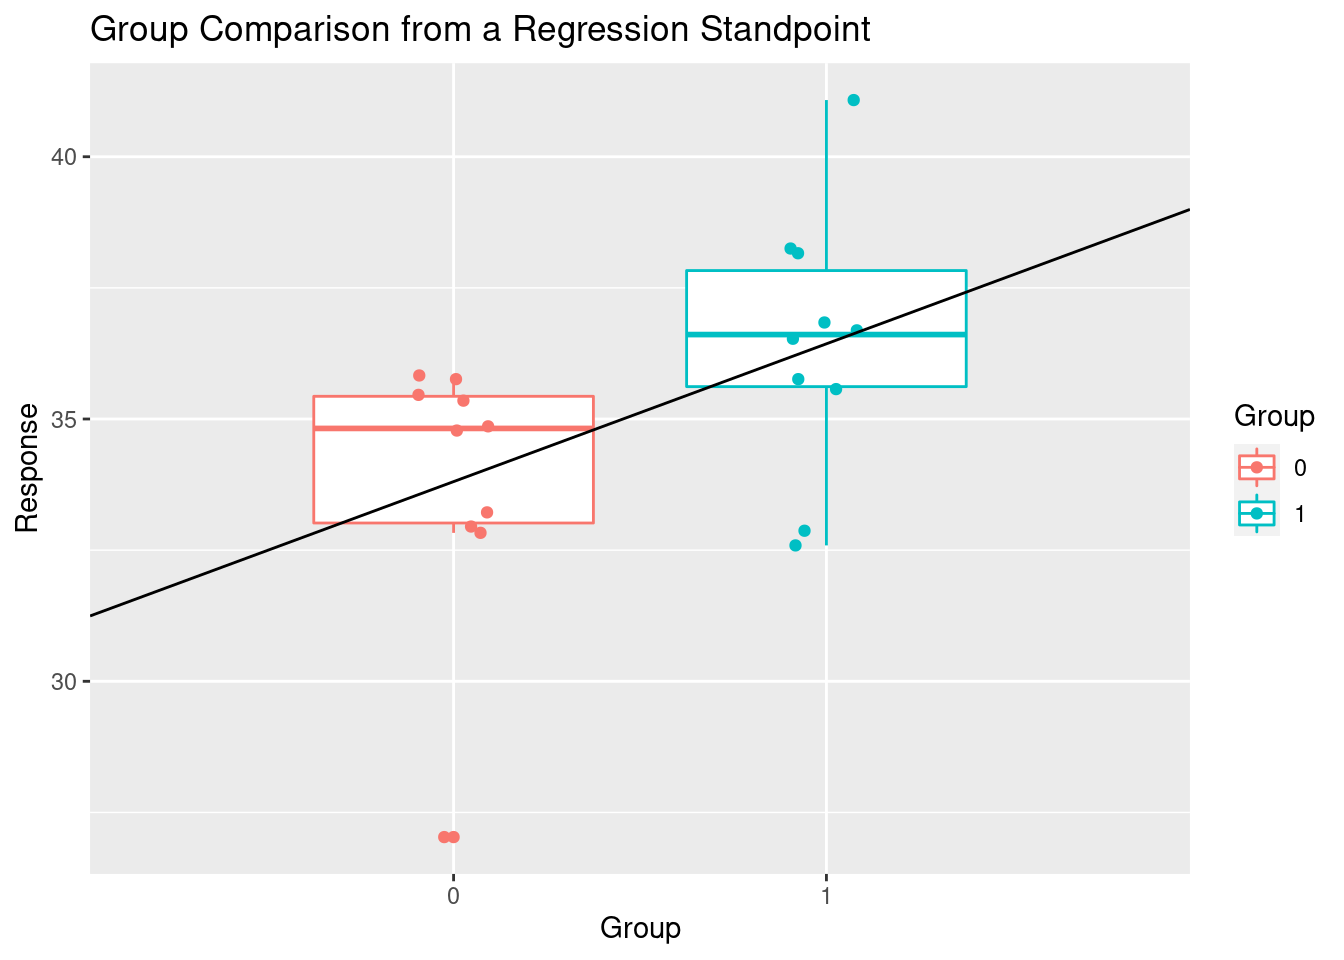
\includegraphics{ANOVA-and-Regression_files/figure-latex/unnamed-chunk-12-1.pdf}

The way you code your categorical variables in a linear model is
extremely important. Different codings lead to different interpretations
of the parameters (betas) in your model. For us, our model is
\[
Y_i = \beta_0+\beta_{i1}X_{i1}+\epsilon_i
\]

From this, we have
\[
\begin{aligned}
E(Y_i|X_{i1}=0) &=\beta_0 \\
E(Y_i|X_{i1}=1) &=\beta_0 + \beta_1
\end{aligned}
\]

From which we can derive,

\[
\beta_1 = E(Y_i|X_{i1}=1) - E(Y_i|X_{i1}=0)
\]

So, our slope estimate is the estimated amount by which the mean of
group1 is above that of the mean of group0.

Run linear regression

\begin{Shaded}
\begin{Highlighting}[]
\FunctionTok{summary}\NormalTok{(data1\_lm\_independent\_samples)}
\end{Highlighting}
\end{Shaded}

\begin{verbatim}
## 
## Call:
## lm(formula = response ~ group, data = data1)
## 
## Residuals:
##     Min      1Q  Median      3Q     Max 
## -6.7770 -0.8587  0.3310  1.6712  4.6460 
## 
## Coefficients:
##             Estimate Std. Error t value Pr(>|t|)    
## (Intercept)  33.8070     0.8159  41.436   <2e-16 ***
## group         2.6270     1.1538   2.277   0.0352 *  
## ---
## Signif. codes:  0 '***' 0.001 '**' 0.01 '*' 0.05 '.' 0.1 ' ' 1
## 
## Residual standard error: 2.58 on 18 degrees of freedom
## Multiple R-squared:  0.2236, Adjusted R-squared:  0.1805 
## F-statistic: 5.184 on 1 and 18 DF,  p-value: 0.03524
\end{verbatim}

Run ANOVA

\begin{Shaded}
\begin{Highlighting}[]
\NormalTok{data1}\SpecialCharTok{$}\NormalTok{group }\OtherTok{=} \FunctionTok{as.factor}\NormalTok{(data1}\SpecialCharTok{$}\NormalTok{group)}
\NormalTok{data1\_ANOVA\_independent\_samples }\OtherTok{=} \FunctionTok{aov}\NormalTok{(response }\SpecialCharTok{\textasciitilde{}}\NormalTok{ group,}
    \AttributeTok{data =}\NormalTok{ data1)}
\FunctionTok{summary}\NormalTok{(data1\_ANOVA\_independent\_samples)}
\end{Highlighting}
\end{Shaded}

\begin{verbatim}
##             Df Sum Sq Mean Sq F value Pr(>F)  
## group        1  34.51   34.51   5.184 0.0352 *
## Residuals   18 119.82    6.66                 
## ---
## Signif. codes:  0 '***' 0.001 '**' 0.01 '*' 0.05 '.' 0.1 ' ' 1
\end{verbatim}

Run t-Test

\begin{Shaded}
\begin{Highlighting}[]
\NormalTok{(}\AttributeTok{data1\_t\_test\_independent\_samples =} \FunctionTok{t.test}\NormalTok{(}\AttributeTok{x =}\NormalTok{ data1[data1}\SpecialCharTok{$}\NormalTok{group }\SpecialCharTok{==}
    \DecValTok{1}\NormalTok{, }\StringTok{"response"}\NormalTok{], }\AttributeTok{y =}\NormalTok{ data1[data1}\SpecialCharTok{$}\NormalTok{group }\SpecialCharTok{==} \DecValTok{0}\NormalTok{, }\StringTok{"response"}\NormalTok{],}
    \AttributeTok{paired =} \ConstantTok{FALSE}\NormalTok{, }\AttributeTok{var.equal =} \ConstantTok{TRUE}\NormalTok{))}
\end{Highlighting}
\end{Shaded}

\begin{verbatim}
## 
##  Two Sample t-test
## 
## data:  data1[data1$group == 1, "response"] and data1[data1$group == 0, "response"]
## t = 2.2768, df = 18, p-value = 0.03524
## alternative hypothesis: true difference in means is not equal to 0
## 95 percent confidence interval:
##  0.2029061 5.0510939
## sample estimates:
## mean of x mean of y 
##    36.434    33.807
\end{verbatim}

Notice the similarities.

\begin{Shaded}
\begin{Highlighting}[]
\CommentTok{\# Confidence interval for the difference in the}
\CommentTok{\# means}
\FunctionTok{confint}\NormalTok{(data1\_lm\_independent\_samples, }\StringTok{"group"}\NormalTok{, }\AttributeTok{level =} \FloatTok{0.95}\NormalTok{)}
\end{Highlighting}
\end{Shaded}

\begin{verbatim}
##           2.5 %   97.5 %
## group 0.2029061 5.051094
\end{verbatim}

\begin{Shaded}
\begin{Highlighting}[]
\NormalTok{data1\_t\_test\_independent\_samples}\SpecialCharTok{$}\NormalTok{conf.int}
\end{Highlighting}
\end{Shaded}

\begin{verbatim}
## [1] 0.2029061 5.0510939
## attr(,"conf.level")
## [1] 0.95
\end{verbatim}

\begin{Shaded}
\begin{Highlighting}[]
\CommentTok{\# p{-}values}
\FunctionTok{with}\NormalTok{(}\FunctionTok{summary}\NormalTok{(data1\_lm\_independent\_samples), }\FunctionTok{unname}\NormalTok{(}\FunctionTok{pf}\NormalTok{(fstatistic[}\DecValTok{1}\NormalTok{],}
\NormalTok{    fstatistic[}\DecValTok{2}\NormalTok{], fstatistic[}\DecValTok{3}\NormalTok{], }\AttributeTok{lower.tail =}\NormalTok{ F)))}
\end{Highlighting}
\end{Shaded}

\begin{verbatim}
## [1] 0.03524354
\end{verbatim}

\begin{Shaded}
\begin{Highlighting}[]
\FunctionTok{summary}\NormalTok{(data1\_ANOVA\_independent\_samples)[[}\DecValTok{1}\NormalTok{]][[}\DecValTok{1}\NormalTok{, }\DecValTok{5}\NormalTok{]]}
\end{Highlighting}
\end{Shaded}

\begin{verbatim}
## [1] 0.03524354
\end{verbatim}

\begin{Shaded}
\begin{Highlighting}[]
\NormalTok{data1\_t\_test\_independent\_samples}\SpecialCharTok{$}\NormalTok{p.value}
\end{Highlighting}
\end{Shaded}

\begin{verbatim}
## [1] 0.03524354
\end{verbatim}

Now, let's look at something else. The CO2 data frame has 84 rows and 5
columns of data from an experiment on the cold tolerance of the grass
species Echinochloa crus-galli.

\begin{Shaded}
\begin{Highlighting}[]
\FunctionTok{data}\NormalTok{(}\StringTok{"CO2"}\NormalTok{)}
\NormalTok{CO2[}\FunctionTok{sample}\NormalTok{(}\FunctionTok{nrow}\NormalTok{(CO2), }\AttributeTok{size =} \DecValTok{5}\NormalTok{), ]}
\end{Highlighting}
\end{Shaded}

\begin{verbatim}
##    Plant        Type  Treatment conc uptake
## 70   Mc1 Mississippi    chilled 1000   21.9
## 84   Mc3 Mississippi    chilled 1000   19.9
## 75   Mc2 Mississippi    chilled  500   12.5
## 81   Mc3 Mississippi    chilled  350   17.9
## 13   Qn2      Quebec nonchilled  675   41.4
\end{verbatim}

What is a linear model? In the context of linear regression, a linear
model is a relationship between the responses and the explanatory
variables that is linear in the parameters.

\begin{Shaded}
\begin{Highlighting}[]
\NormalTok{CO2\_recipe }\OtherTok{=} \FunctionTok{recipe}\NormalTok{(uptake }\SpecialCharTok{\textasciitilde{}}\NormalTok{ ., }\AttributeTok{data =}\NormalTok{ CO2) }\SpecialCharTok{\%\textgreater{}\%}
    \FunctionTok{step\_dummy}\NormalTok{(}\FunctionTok{c}\NormalTok{(}\StringTok{"Type"}\NormalTok{, }\StringTok{"Treatment"}\NormalTok{))}
\CommentTok{\# see contrasts() function}
\NormalTok{CO2\_linear\_model }\OtherTok{=} \FunctionTok{linear\_reg}\NormalTok{() }\SpecialCharTok{\%\textgreater{}\%}
    \FunctionTok{set\_engine}\NormalTok{(}\StringTok{"lm"}\NormalTok{, }\AttributeTok{contrasts =} \FunctionTok{list}\NormalTok{(}\AttributeTok{Plant =} \StringTok{"contr.poly"}\NormalTok{))}
\NormalTok{CO2\_workflow }\OtherTok{=} \FunctionTok{workflow}\NormalTok{() }\SpecialCharTok{\%\textgreater{}\%}
    \FunctionTok{add\_model}\NormalTok{(CO2\_linear\_model) }\SpecialCharTok{\%\textgreater{}\%}
    \FunctionTok{add\_recipe}\NormalTok{(CO2\_recipe)}
\NormalTok{CO2\_fit }\OtherTok{=}\NormalTok{ CO2\_workflow }\SpecialCharTok{\%\textgreater{}\%}
    \FunctionTok{fit}\NormalTok{(}\AttributeTok{data =}\NormalTok{ CO2)}
\end{Highlighting}
\end{Shaded}

\begin{Shaded}
\begin{Highlighting}[]
\NormalTok{CO2\_fit }\SpecialCharTok{\%\textgreater{}\%}
    \FunctionTok{pull\_workflow\_fit}\NormalTok{() }\SpecialCharTok{\%\textgreater{}\%}
    \FunctionTok{tidy}\NormalTok{()}
\end{Highlighting}
\end{Shaded}

\begin{verbatim}
## # A tibble: 15 x 5
##    term              estimate std.error statistic   p.value
##    <chr>                <dbl>     <dbl>     <dbl>     <dbl>
##  1 (Intercept)        19.5      1.17      16.7     2.96e-26
##  2 Plant.L           -22.9      2.27     -10.1     2.17e-15
##  3 Plant.Q            -4.62     2.27      -2.03    4.57e- 2
##  4 Plant.C             4.67     2.27       2.06    4.34e- 2
##  5 Plant^4             2.34     2.27       1.03    3.06e- 1
##  6 Plant^5             4.31     2.27       1.90    6.13e- 2
##  7 Plant^6            -0.0390   2.27      -0.0172  9.86e- 1
##  8 Plant^7            -2.04     2.27      -0.897   3.73e- 1
##  9 Plant^8            -3.28     2.27      -1.44    1.53e- 1
## 10 Plant^9            -9.07     2.27      -4.00    1.56e- 4
## 11 Plant^10            0.546    2.27       0.241   8.10e- 1
## 12 Plant^11            1.91     2.27       0.843   4.02e- 1
## 13 conc                0.0177   0.00223    7.96    1.97e-11
## 14 Type_Mississippi   NA       NA         NA      NA       
## 15 Treatment_chilled  NA       NA         NA      NA
\end{verbatim}

\printbibliography

\end{document}
